%**************************************************************************
%* SpringSim 2017 Author Kit
%*
%* Word Processing System: TeXnicCenter and MiKTeX
%*
%**************************************************************************

\documentclass{scspaperproc}

\usepackage{latexsym}
\usepackage{graphicx}
\usepackage{mathptmx}
\usepackage{amsmath}
\usepackage{amsfonts}
\usepackage{amssymb}
\usepackage{amsbsy}
\usepackage{amsthm}
%% \usepackage{color}   % Needed to color text for drafts

%% \usepackage{algorithm}     % needed for the algorithm block
%% \usepackage{algpseudocode} % algorithmicx psuedo-code styling
%\usepackage[pdftex,colorlinks=true,urlcolor=blue,citecolor=black,anchorcolor=black,linkcolor=black]{hyperref}
%% \usepackage[dvips,colorlinks=true,urlcolor=blue,citecolor=black,%
%% anchorcolor=black,linkcolor=black]{hyperref}

% custom hyphenation rules
\usepackage{hyphenat}
\hyphenation{op-tical net-works semi-conduc-tor}

% theorem style
\newtheoremstyle{scsthe}% hnamei
{8pt}% hSpace abovei
{8pt}% hSpace belowi
{\it}% hBody fonti
{}% hIndent amounti1
{\bf}% hTheorem head fontbf
{.}% hPunctuation after theorem headi
{.5em}% hSpace after theorem headi2
{}% hTheorem head spec (can be left empty, meaning `normal')i
\theoremstyle{scsthe}
\newtheorem{theorem}{Theorem}
\renewcommand{\thetheorem}{\arabic{theorem}}
\newtheorem{corollary}[theorem]{Corollary}
\renewcommand{\thecorollary}{\arabic{corollary}}
\newtheorem{definition}{Definition}
\renewcommand{\thedefinition}{\arabic{definition}}
\newcommand{\rpm}{\raisebox{.2ex}{$\scriptstyle\pm$}}

% avoid overrunning the right margin
\sloppy

%% ***** NOTE *****

%% The use of the long citation format (e.g. "Brown and Edwards
%% (1993)" rather than "[5]") and at the same time using the hyperref
%% package can lead to hard to trace bugs in case the citation is
%% broken accross the line (usually this will mark the entire
%% paragraph as a hyperlink (clickable) which is easily noticeable and
%% fixed if using colorlinks, but not if the color is black -- as it
%% is now). Worse yet, if a citation spans page boundary, LaTeX
%% compilation can fail, with an obscure error message. Since this
%% depends a lot on the flow of the text and wording, these bugs come
%% and go and can be extremely hard for a beginner to trace. The error
%% message can look like this:
%%
%%    ! pdfTeX error (ext4): \pdfendlink ended up in different nesting
%%    level than \pdfstartlink.  \AtBegShi@Output ...ipout \box
%%    \AtBeginShipoutBox \fi \fi
%%    l.174 
%%    ! ==> Fatal error occurred, no output PDF file produced!
%%
%% and can be universally fixed by putting an \mbox{} around the
%% citation in question (in this case, at line 174) and maybe adapting
%% the wording a little bit to improve the paragraph typesetting,
%% which is perhaps not immediately obvious.
%****************************************************************************

% begin document
\begin{document}

% Page header (author list)
\SCSpagesetup{Lux, Watson, Chang, Bernard, Li, Xu, Back, Butt, Cameron, and Hong}

% Conference info
\def\SCSconferenceacro{SpringSim}
\def\SCSpublicationyear{2018}
\def\SCSconferencedates{April 15-18}
\def\SCSconferencevenue{Baltimore, MD, USA}
\def\SCSsymposiumacro{HPC} % High Performance Computing Symposium

% title
\title{Predictive Modeling of I/O Characteristics \\ in High
  Performance Computing Systems}

% AUTHOR LIST
% *** NOTE: May need to adjust titlevboxsize in the preamble
\author{Thomas C. H. Lux \\ [8pt]
Dept. of Computer Science \\
Virginia Polytechnic Institute\\
\& State University (VPI\&SU) \\
Blacksburg, VA 24061 \\
tchlux@vt.edu \\
\and
Layne T. Watson \\[8pt]
Dept. of Computer Science\\
Dept. of Mathematics\\
Dept. of Aerospace \& Ocean Eng.\\ 
VPI \& SU \\
\and
\vspace{-30pt}\\
Tyler H. Chang\\ [8pt]
Dept. of Computer Science \\
VPI \& SU \\
}

\maketitle

\vspace{-20pt}

Additional authors are listed in the Additional Authors section.

\section*{Abstract}

Each of high performance computing, cloud computing, and computer
security have their own interests in modeling and predicting the
performance of computers with respect to how they are configured. An
effective model might infer internal mechanics, minimize power
consumption, or maximize computational throughput of a given
system. This paper analyzes a four-dimensional dataset measuring the
input/output (I/O) characteristics of a cluster of identical computers
using the benchmark IOzone. The I/O performance characteristics are
modeled with respect to system configuration using multivariate
interpolation and approximation techniques. The analysis reveals that
accurate models of I/O characteristics for a computer system may be
created from a small fraction of possible configurations, and that
some modeling techniques will continue to perform well as the number
of system parameters being modeled increases. These results have
strong implications for future predictive analyses based on more
comprehensive sets of system parameters.

\textbf{Keywords:} Regression, approximation, interpolation,
performance modeling


%     Introduction     
%======================
\section{Introduction and related work}
\label{sec:introduction}

Performance tuning is often an experimentally complex and time
intensive chore necessary for configuring HPC systems. The procedures
for this tuning vary largely from system to system and are often
subjectively guided by the system engineer(s). Once a desired level of
performance is achieved, an HPC system may only be incrementally
reconfigured as required by updates or specific jobs. In the case that
a system has changing workloads or nonstationary performance
objectives that range from maximizing computational throughput to
minimizing power consumption and system variability, it becomes clear
that a more effective and automated tool is needed for configuring
systems. This scenario presents a challenging and important
application of multivariate approximation and interpolation
techniques.

Predicting the performance of an HPC system is a challenging problem
that is primarily attempted in one of two ways: (1) build a
statistical model of the performance by running experiments on the
system at select settings, or (2) run artificial experiments using a
simplified simulation of the target system to estimate architecture
and application bottlenecks. In this paper the proposed multivariate
modeling techniques rest in the first category, and they represent a
notable increase in the ability to model complex interactions between
system parameters.

Many previous works attempting to model system performance have used
simulated environments to estimate the performance of a system
\shortcite{grobelny2007fase,wang2009simulation,wang2013towards}. Some
of these works refer to statistical models as being oversimplified and
not capable of capturing the true complexity of the underlying
system. This claim is partially correct, noting that a large portion
of predictive statistical models rely on simplifying the model to one
or two parameters
\shortcite{snavely2002framework,bailey2005performance,barker2009using,ye2010analyzing}.
These limited statistical models have provided satisfactory
performance in very narrow application settings. Many of the
aforementioned statistical modeling techniques claim to generalize,
while simultaneously requiring additional code annotations, hardware
abstractions, or additional application level understandings in order
to generate models. The approach presented here requires no
modifications of the application, no architectural abstractions, nor
any structural descriptions of the input data being modeled. The
techniques used are purely mathematical and only need performance data
as input.

Among the statistical models presented in prior works,
\shortciteN{bailey2005performance} specifically mention that it is
difficult for the simplified models to capture variability introduced
by I/O. System variability in general has become a problem of
increasing interest to the HPC and systems communities, however most
of the work has focused on operating system (OS) induced variability
\shortcite{beckman2008benchmarking,de2007identifying}. The work that
has focused on managing I/O variability does not use any sophisticated
modeling techniques \shortcite{lofstead2010managing}. Hence, this
paper presents a case study applying advanced mathematical and
statistical modeling techniques to the domain of HPC I/O
characteristics. The models are used to predict the mean throughput of
a system and the variance in throughput of a system. The discussion
section outlines how the techniques presented can be applied to any
performance metric and any system.

%% Multivariate models for an HPC system would be a function of the
%% tunable parameters built to accurately model some desired performance
%% metric.

%% \begin{enumerate}
%% \item The value of multivariate Modeling
%% \item The data context
%% \item The proposed method for using multivariate models
%% \item The impact of effective models
%% \end{enumerate}

In general, this paper compares five multivariate approximation
techniques that operate on inputs in $\mathbb{R}^d$ ($d$-tuples of
real numbers) and produce predicted responses in $\mathbb{R}$. In
order to provide coverage of the varied mathematical strategies that
can be employed to solve the continuous modeling problem, three of the
techniques are regression based and the remaining two are
interpolants. The sections below outline the mathematical formulation
of each technique and provide computational complexity bounds with
respect to the size (number of points and dimension) of input
data. Throughout, $d$ will refer to the dimension of the input data,
$n$ is the number of points in the input data, $x^{(i)} \in
\mathbb{R}^d$ is the $i$-th input data point, $x^{(i)}_j$ is the
$j$-th component of $x^{(i)}$, and $f(x^{(i)})$ is the response value
of the $i$-th input data point.

The remainder of the paper is broken up into five major parts. Section
\ref{sec:multivariate} provides an overview of the multivariate
modeling techniques, Section \ref{sec:methodology} outlines the
methodology for comparing and evaluating the performance of the
models, Section \ref{sec:results} presents the IOzone predictions,
Section \ref{sec:discussion} discusses the obvious and subtle
implications of the models' performance, and Section
\ref{sec:conclusion} concludes and offers directions for future work.

\section{Multivariate Models}
\label{sec:multivariate}

\subsection{Regression}
\vspace{-10pt}
Multivariate approximations are capable of accurately modeling a
complex dependence of a response (in $\mathbb{R}$) on multiple
variables (represented as a points in $\mathbb{R}^{d}$). The
approximations to some (unknown) underlying function $f: \mathbb{R}^d
\rightarrow \mathbb{R}$ are chosen to minimize some error measure
related to data samples $f(x^{(i)})$. For example, least squares
regression uses the sum of squared differences between modeled
response values and true response values as an error measure.

\vspace{-10pt}
\subsubsection{Multivariate Adaptive Regression Splines}
\vspace{-10pt}
This approximation was introduced in
\shortciteN{friedman1991multivariate} and subsequently improved to its
current version in \shortciteN{stanford1993fast}, called fast
multivariate adaptive regression splines (Fast MARS). In Fast MARS, a
least squares fit model is iteratively built by beginning with a
single constant valued function and adding two new basis functions at
each iteration of the form

$$ B_{2s-1}(x) = B_l(x) [c(x_i-v)]_+ ,$$
$$ B_{2s}(x) = B_k(x) [c(x_i-v)]_- ,$$

where $s$ is the iteration number, $B_l(x)$ and $B_k(x)$ are basis
functions from the previous iteration, $c, v \in \mathbb{R}$, 

$$w_+ = \begin{cases} w, & w \geq 0 \\ 0, & w < 0 \end{cases},$$

and $w_- = (-w)_+$. After iteratively constructing a model, MARS then
iteratively removes basis functions that do not contribute to goodness
of fit. In effect, MARS creates a locally component-wise tensor
product approximation of the data. The overall computational
complexity of Fast MARS is $\mathcal{O}(n d m^3)$ where $m$ is the
maximum number of underlying basis functions. This paper uses an
implementation of Fast MARS \shortcite{rudy2017pyearth} with $m =
200$.

\vspace{-10pt}
\subsubsection{Multilayer Perceptron Regressor}
\vspace{-10pt}
The neural network is a well studied and widely used method for both
regression and classification tasks
\shortcite{hornik1989multilayer}. When using the rectified linear unit
(ReLU) activation function \shortcite{dahl2013improving} and training
with the BFGS minimization technique \shortcite{moller1993scaled}, the
model built by a multilayer perceptron uses layers $l : \mathbb{R}^{i}
\rightarrow \mathbb{R}^{j}$ defined by

$$ l(u) = \big( u^t W_l \big)_+ ,$$

where $W_l$ is the $i$ by $j$ weight matrix for layer $l$. In this
form, the multilayer perceptron (MLP) produces a piecewise linear
model of the input data. The computational complexity of training a
multilayer perceptron is $\mathcal{O}(n d m)$, where $m$ is
determined by the sizes of the layers of the network and the stopping
criterion of the BFGS minimization used for finding weights. This
paper uses the scikit-learn MLP regressor \shortcite{scikit-learn}, a
single hidden layer with 100 nodes, ReLU activation, and BFGS for
training.

\subsubsection{Support Vector Regressor}
\vspace{-10pt}
Support vector machines are a common method used in machine learning
classification tasks that can be adapted for the purpose of regression
\shortcite{basak2007support}. How to build a support vector regressor
(SVR) is beyond the scope of this summary, but the resulting
functional fit $p : \mathbb{R}^d \rightarrow \mathbb{R}$ has the form

$$ p(x)  = \sum_{i=1}^{n}a_i K(x,x^{(i)}) + b ,$$

%% $$ \text{Minimize } \bigg\{ \frac{1}{2}\sum_{i=1}^{n}\sum_{j=1}^{n}
%% a_i a_j K(x_i, x_j) + \epsilon \sum_{i=1}^{n} a_i - \sum_{i=1}^{n} y_i
%% a_i \bigg\} $$

%% $$ \text{Subject to } \sum_{i=1}^{n}a_i = 0 \text{ } \text{ and }
%% \text{ } a_i \in [0,C] $$

where $K$ is the selected kernel function, $a \in \mathbb{R}^n$, $b
\in \mathbb{R}$ are coefficients to be solved for simultaneously. The
computational complexity of the SVR is $\mathcal{O}(n^2dm)$, with $m$
being determined by the minimization convergence criterion. This paper
uses the scikit-learn SVR \shortcite{scikit-learn} with a polynomial
kernel function.

\vspace{-10pt}
\subsection{Interpolation}
\vspace{-10pt}
In some cases it is desirable to have a model that can recreate the
input data exactly. This is especially the case when the confidence in
the response values for known data is high. Both interpolation models
analyzed in this paper are based on linear functions.

\vspace{-10pt}
\subsubsection{Delaunay}
\vspace{-10pt}
The Delaunay method of interpolation is a well studied geometric
technique for producing an interpolant \shortcite{lee1980two}. The
Delaunay triangulation of a set of data points into simplices is such
that the sphere defined by the vertices of each simplex contains no
data points in the sphere's interior. For a $d$-simplex S with
vertices $v^{(0)}$, $v^{(1)}$, $\ldots$, $v^{(d)}$, $x \in S$, and
data values $f(v^{(i)})$, $i=0$, $\ldots$, $d$, $x$ is a unique convex
combination of the vertices,

$$ x = \sum_{i=0}^{d} w_i v^{(i)}, \quad \sum_{i=0}^{d} w_i = 1, \quad
w_i \geq 0, \quad i=0,\ldots,d ,$$

and the Delaunay interpolant to $f$ at $x$ is given by

$$ p(x) = \sum_{i=0}^{d} w_i f(v^{(i)}). $$

The computational complexity of the Delaunay triangulation (for the
implementation used here) is $\mathcal{O}(n^{\lceil d/2 \rceil})$,
which is not scalable to $d > 10$ \shortcite{sartipizadeh2016computing}.
The scipy interface \shortcite{scipy} to the QuickHull implementation
\shortcite{barber1996qhull} of the Delaunay triangulation is used here.

\subsubsection{Linear Shepard}
\vspace{-10pt}
The linear Shepard method (LSHEP) is a blending function using local
linear interpolants, a special case of the general Shepard algorithm
\shortcite{thacker2010algorithm}. The interpolant has the form

$$ p(x) = \frac{\sum_{k=1}^{n}W_k(x)P_k(x)}{\sum_{k=1}^{n}W_k(x)} ,$$

where $W_k(x)$ is a locally supported weighting function and $P_k(x)$
is a local linear approximation to the data satisfying
$P_k\big(x^{(k)}\big) = f\big(x^{(x)}\big)$. The computational
complexity of LSHEP is $\mathcal{O}(n^2d^3)$. This paper uses the
Fortran\#95 implementation of LSHEP in SHEPPACK
\shortcite{thacker2010algorithm}.

%% %     Related Work     
%% %======================
%% \section{Related Work}
%% \begin{enumerate}
%% \item Not sure how much to include here? Shooting for thoroughness or
%%   simply necessary coverage? How much background should I expect the
%%   readers of this paper to have in the ``multivariate modeling of
%%   systems'' area?
%% \end{enumerate}

%     Methodology     
%=====================
\section{Methodology}
\label{sec:methodology}
\subsection{Data}
\vspace{-10pt}

In order to evaluate the viability of multivariate models for
predicting system performance, this paper presents a case study of a
four-dimensional dataset produced by executing the IOzone benchmark
from \shortciteN{iozone} on a homogeneous cluster of computers. All
experiments were performed on parallel shared-memory nodes common to
HPC systems. Each system had a lone guest Linux operating system
(Ubuntu 14.04 LTS//XEN 4.0) on a dedicated 2TB HDD on a 2 socket, 4
core (2 hyperthreads per core) Intel Xeon E5-2623 v3 (Haswell)
platform with 32 GB DDR4. The system performance data was collected by
executing IOzone 40 times for each of a select set of system
configurations. A single IOzone execution reports the max I/O
throughput seen for the selected test in kilobytes per second. The 40
executions for each system configuration are converted into the mean
and variance, both values in $\mathbb{R}$ capable of being modeled
individually by the multivariate approximation techniques presented in
Section \ref{sec:multivariate}. The summary of data used in the
experiments for this paper can be seen in Table \ref{tab:data_type}.
Distributions of raw throughput values being modeled can be seen in
Figure \ref{fig:raw_throughput}.

\begin{table}
  \centering
  \begin{tabular}{c|c}
    \hline
    \textbf{System Parameter} & \textbf{Values}\\
    \hline
    File Size & 64, 256, 1024\\
    Record Size & 32, 128, 512\\
    Thread Count & 1, 2, 4, 8, 16, 32, 64, 128, 256\\
    Frequency & \{12, 14, 15, 16, 18, 19, 20, 21, 23, 24, 25, 27, 28, 29, 30, 30.01\} $\times 10^5$\\
    \hline
    \textbf{Response Values} & \\
    \hline
    Throughput Mean & [$2.6 \times 10^5$, $5.9 \times 10^8$]\\
    Throughput Variance & [$5.9\times 10^{10} $, $4.7 \times 10^{16}$]\\
    \hline
  \end{tabular}
  \caption{A description of the system parameters being considered in
    the IOzone tests. Record size must not be greater than file size
    and hence there are only six valid combinations of the two. In
    total there are $6 \times 9 \times 16 = 864$ unique system
    configurations.}
  \label{tab:data_type}
\end{table}

\begin{figure}
  \centering
  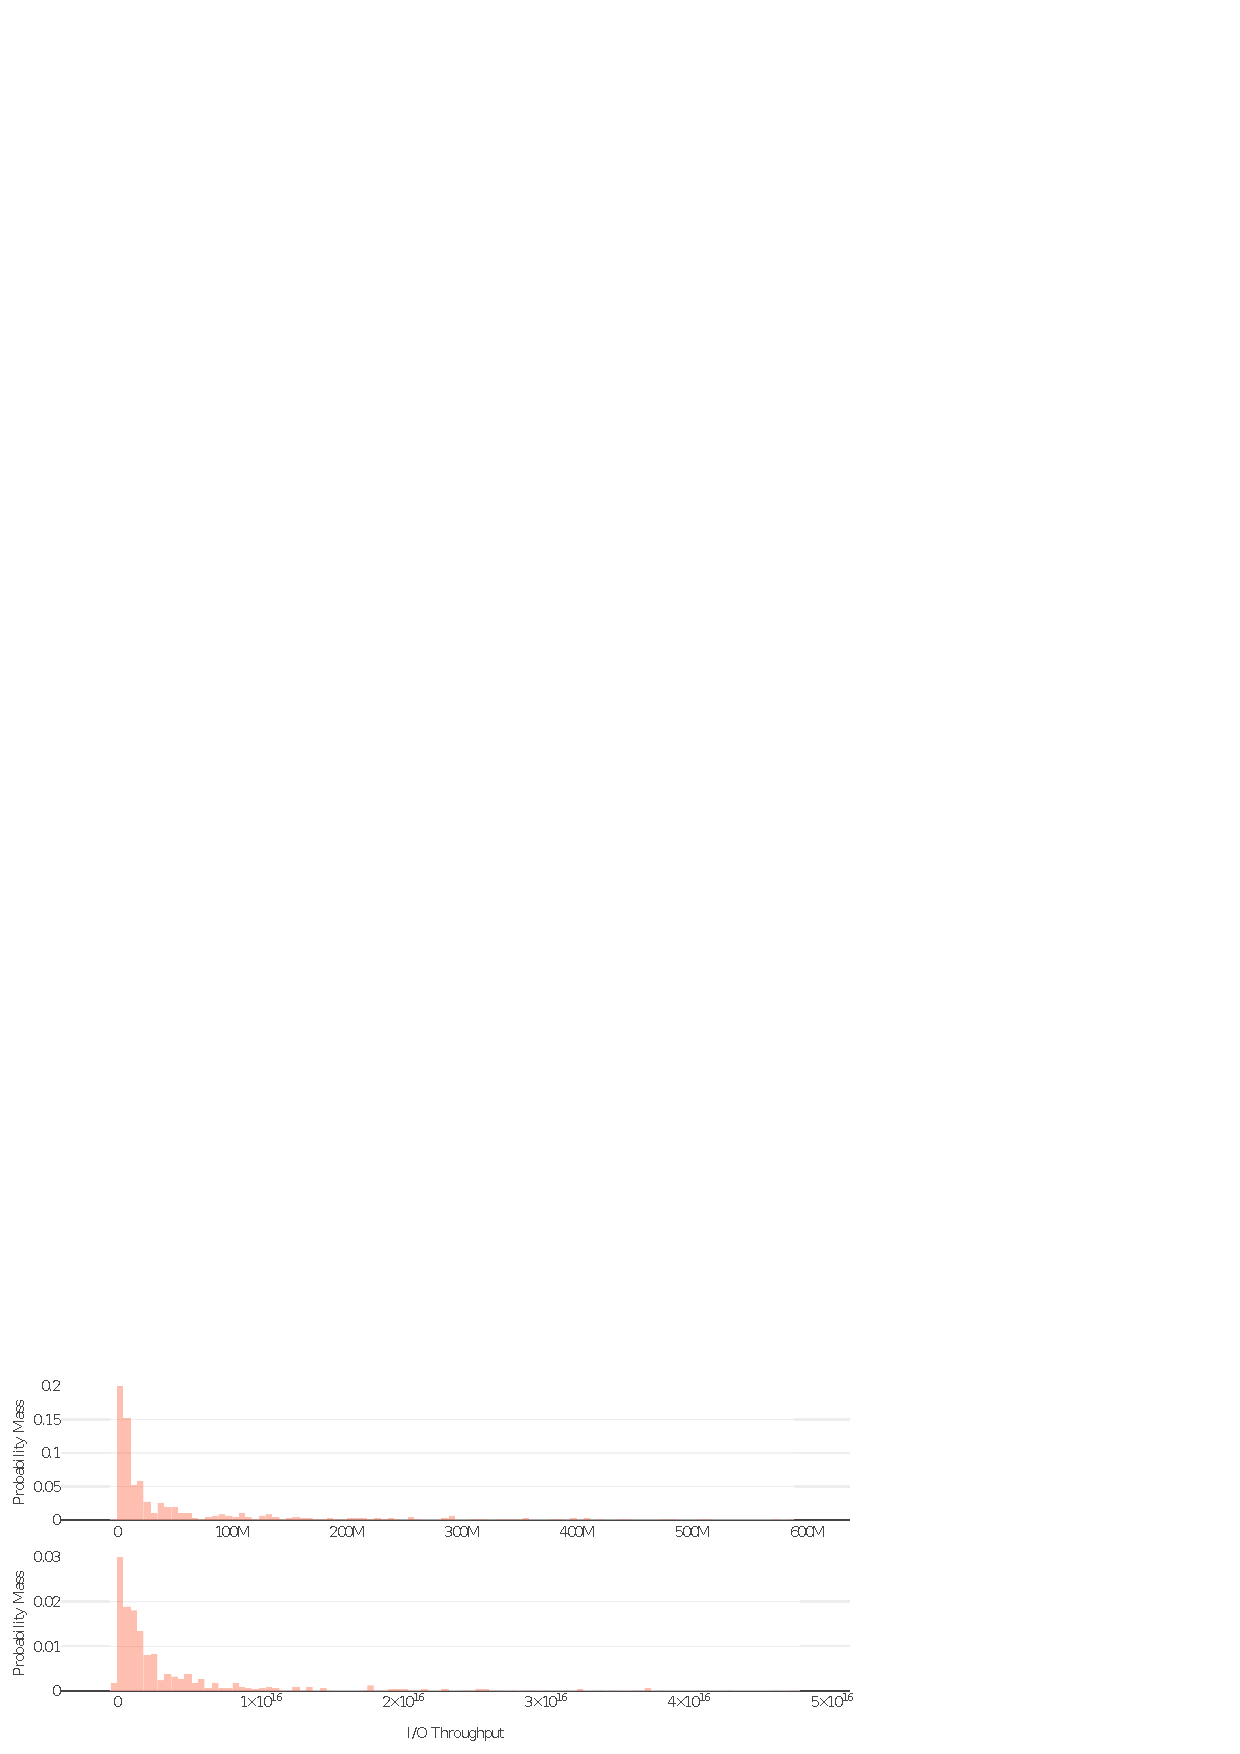
\includegraphics[width=\textwidth,trim={0 .5in 0 .4in}]{Raw_Throughput.pdf}
  \caption{Histograms of 100-bin reductions of the PMF of I/O
    throughput mean (top) and I/O throughput variance (bottom). In the
    mean plot, the first 1\% bin (truncated in plot) has a probability
    mass of .45. In the variance plot, the second 1\% bin has a
    probability mass of .58. It can be seen that the distributions of
    throughputs are primarily of lower magnitude with occasional
    extreme outliers.}
  \label{fig:raw_throughput}
\end{figure}

\vspace{-10pt}
\subsection{Dimensional Analysis}
\vspace{-10pt}
This work utilizes an extension to standard $k$-fold cross validation
that allows for a more thorough investigation of the expected model
performance in a variety of real-world situations. Alongside
randomized splits, two extra components are considered: the amount of
training data provided, and the dimension of the input data. It is
important to consider that algorithms that perform well with less
training input also require less experimentation. Although, the amount
of training data required may change as a function of the dimension of
the input and this needs to be studied as well. The framework used
here will be referred to as a multidimensional analysis (MDA) of the
IOzone data.

%% \color{red}

\subsubsection{Multidimensional Analysis}
\vspace{-10pt}
This procedure combines random selection of training and testing
splits with changes in the input dimension and the ratio of training
size to testing size. Given an input data matrix with $n$ rows
(points) and $d$ columns (components), MDA proceeds as follows:
\begin{enumerate}
\item For all $k = 1$, $\ldots$, $d$ and for all nonempty subsets $F
  \subset \{1, 2, \ldots, d\}$, reduce the input data to points $(z,
  f_F(z))$ with $z \in \mathbb{R}^k$ and $f_F(z) = E\bigl[ \bigl\{
    f\bigl(x^{(i)}\bigr) \bigm| \bigl(x^{(i)}_F = z\bigr) \bigr\}
    \bigr]$, where $E[\cdot]$ denotes the mean and $x^{(i)}_F$ is the
  subvector of $x^{(i)}$ indexed by $F$.
\item For all $r$ in $\{5, 10, \ldots, 95\}$, generate $N$ random
  splits $(train, test)$ of the reduced data with $r$ percentage for
  training and $100 - r$ percentage for testing.
\item When generating each of $N$ random $(train, test)$ splits,
  ensure that all points from $test$ are in the convex hull of points
  in $train$ (to prevent extrapolation); also ensure that the points
  in $train$ are well spaced.
\end{enumerate}

In order to ensure that the testing points are in the convex hull of
the training points, the convex hull vertices of each set of (reduced
dimension) points are forcibly placed in the training set. In order to
ensure that training points are well spaced, a statistical method for
picking points from \shortciteN{amos2014algorithm} is used:
\begin{enumerate}
\item Generate a sequence of all pairs of points
  $\bigl(z^{(i_1)},z^{(j_1)}\bigr), \bigl(z^{(i_2)},z^{(j_2)}\bigr),
  \ldots$ sorted by ascending pairwise Euclidean distance between
  points, so that $\bigl|\bigl|z^{(i_k)}-z^{(j_k)}\bigr|\bigr|_2 \leq
  \bigl|\bigl|z^{(i_{k+1})}-z^{(j_{k+1})}\bigr|\bigr|_2$.
\item Sequentially remove points from candidacy until only $|train|$
  remain by randomly selecting one point from the pair
  $\bigl(z^{(i_m)}, z^{(j_m)}\bigr)$ for $m = 1,\ldots$ if both
  $z^{(i_m)}$ and $z^{(j_m)}$ are still candidates for removal.
\end{enumerate}

Given the large number of constraints, level of reduction, and use of
randomness in the MDA procedure, occasionally $N$ unique
training/testing splits may not be created or may not exist. In these
cases, if there are fewer than $N$ possible splits, then
deterministically generated splits are used. Otherwise after $3N$
attempts, only the unique splits are kept for analysis. The MDA
procedure has been implemented in Python\#3 while most regression and
interpolation methods are Fortran wrapped with Python. All randomness
has been seeded for repeatability.

For any index subset $F$ (of size $k$) and selected value of $r$, MDA
will generate up to $N$ multivariate models $f_F(z)$ and predictions
$\hat{f}_F\big(z^{(i)}\big)$ for a point $z^{(i)} \in \mathbb{R}^k$.
There may be fewer than $N$ predictions made for any given
point. Extreme points of the convex hull for the selected index subset
will always be used for training, never for testing. Points that do
not have any close neighbors will often be used for training in order
to ensure well-spacing. Finally, as mentioned before, some index
subsets do not readily generate $N$ unique training and testing
splits. The summary results presented in this work use the median of
the ($N$ or fewer) values $\hat{f}_F(z)$ at each point as the model
estimate for error analysis.

%% is open source, and is freely available at the url
%% \textit{https://github.com/tchlux/VarSys/HPC\_Paper/Code/multi\_dim\_analysis.py}

%% \begin{enumerate}
%% \item Cycling the categorical settings
%% \item Selecting subsets of 1,2,3 up to 4 dimensions
%% \item Cycling different training : testing ratios (5:95 $\rightarrow$ 95:5)
%% \item Generating 200 random training : testing splits
%% \item Ensuring the testing points are on/inside the convex hull of the training.
%% \item Ensuring the training points are well-spaced.
%% \end{enumerate}

%% \subsection{Prediction}
%% \begin{enumerate}
%% \item For each file generated from the dimensional analysis, train on
%%   the training data, evaluate at the testing data points
%% \end{enumerate}

%     Results     
%=================
\section{Results}
\label{sec:results}

A na\"{\i}ve multivariate prediction technique such as nearest
neighbor could experience relative errors in the range $\displaystyle
[0, \big(\max_x f(x) - \min_x f(x)\big) / \min_x f(x) ]$ when modeling
a nonnegative function $f(x)$ from data. The IOzone mean data response
values span three orders of magnitude (as can be seen in Table
\ref{tab:data_type}) while variance data response values span six
orders of magnitude. It is expected therefore, that all studied
multivariate models perform better than a na\"{\i}ve approach,
achieving relative errors strictly less than $10^3$ for throughput
mean and $10^6$ for throughput variance. Ideally, models will yield
relative errors significantly smaller than 1. The time required to
compute thousands of models involved in processing the IOzone data
through MDA was approximately five hours on a CentOS workstation with
an Intel i7-3770 CPU at 3.40GHz. In four dimensions for example, each
of the models could be constructed and evaluated over hundreds of
points in less than a few seconds.

\vspace{-10pt}
\subsection{I/O Throughput Mean}
\vspace{-10pt}
Almost all multivariate models analyzed make predictions with a
relative error less than 1 for most system configurations when
predicting the mean I/O throughput of a system given varying amounts
of training data. The overall best of the multivariate models,
Delaunay, consistently makes predictions with relative error less than
$.05$ (5\% error). In Figure \ref{fig:mean_tt_ratio} it can also be
seen that the Delaunay model consistently makes good predictions even
with as low as 5\% training data (43 of the 864 system configurations)
regardless of the dimension of the data.

\begin{figure}
  \centering
  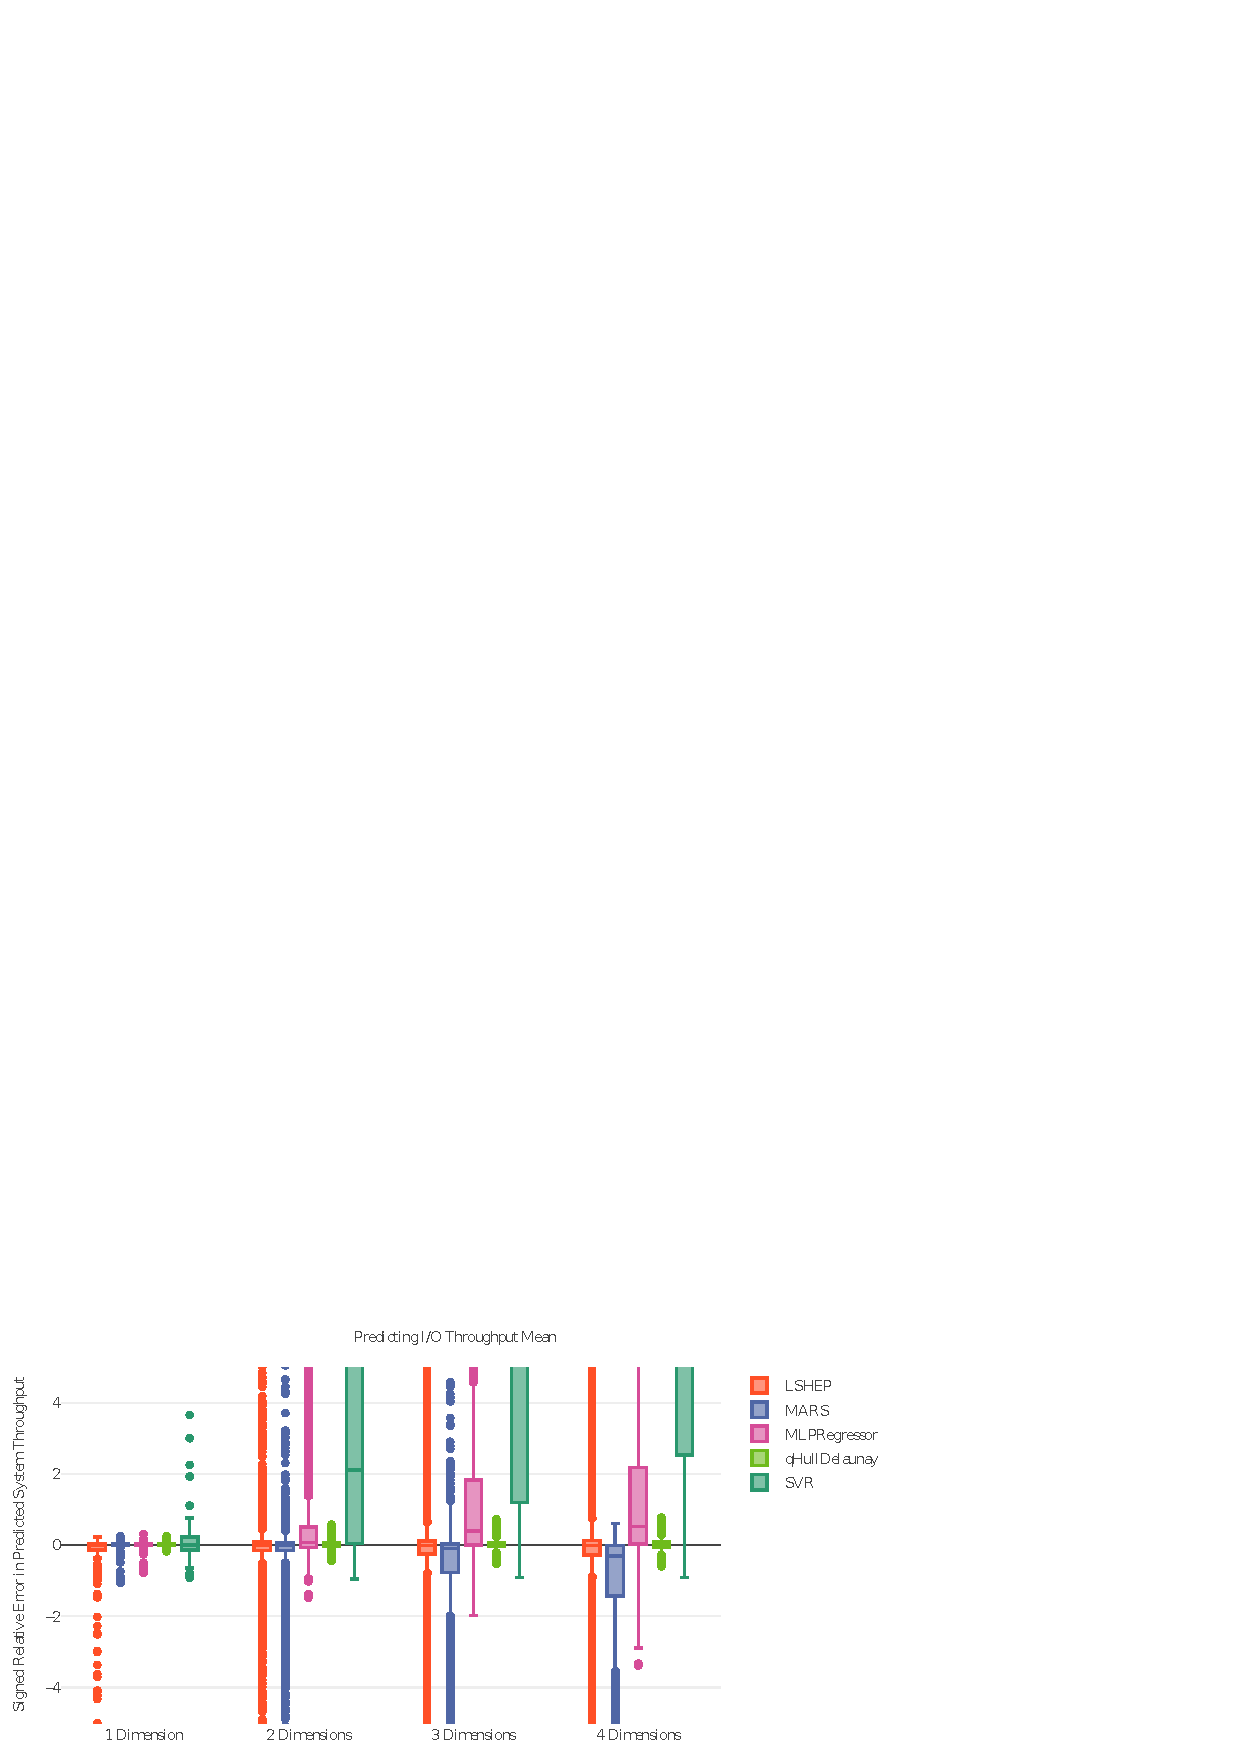
\includegraphics[width=\textwidth,trim={0 .5in 0 .3in}]{Mean_Dim.pdf}
  \caption{These box plots show the prediction error of mean with
    increasing dimension. The top box whisker for SVR is 40, 80, 90
    for dimensions 2, 3, and 4, respectively. Notice that each model
    consistently experiences greater magnitude error with increasing
    dimension. Results for all training percentages are aggregated.}
  \label{fig:mean_dim}
\end{figure}

\begin{figure}
  \centering
  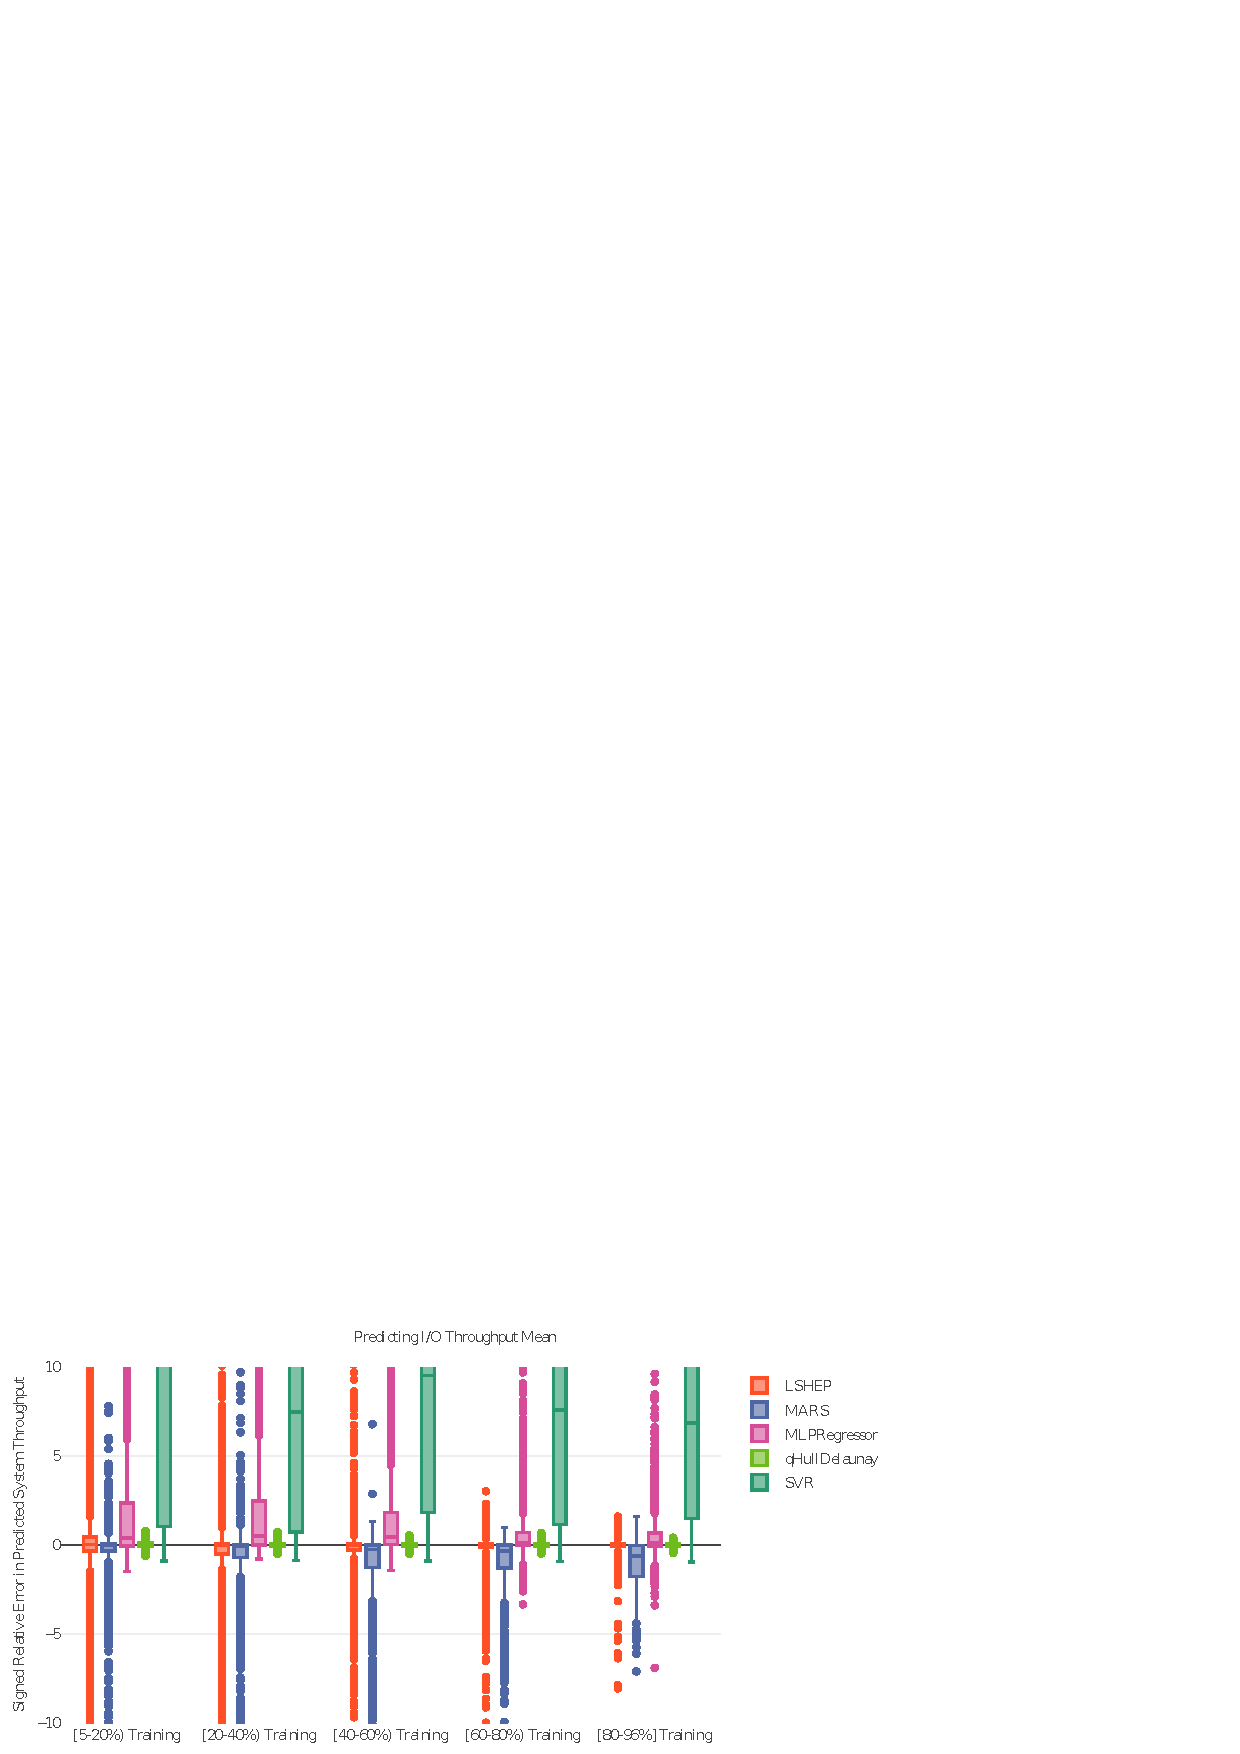
\includegraphics[width=\textwidth,trim={0 .5in 0 .3in}]{Mean_TT_Ratio.pdf}
  \caption{These box plots show the prediction error of mean with
    increasing amounts of training data provided to the models. Notice
    that MARS is the only model whose primary spread of performance
    increases with more training data. Recall that the response values
    being predicted span three orders of magnitude and hence relative
    errors should certainly remain within that range. For SVR the top
    box whisker goes from around 100 to 50 from left to right and is
    truncated in order to maintain focus on better models. Results for
    all dimensions are aggregated. Max training percentage is 96\% due
    to rounding training set size.}
  \label{fig:mean_tt_ratio}
\end{figure}

\begin{figure}
  \centering
  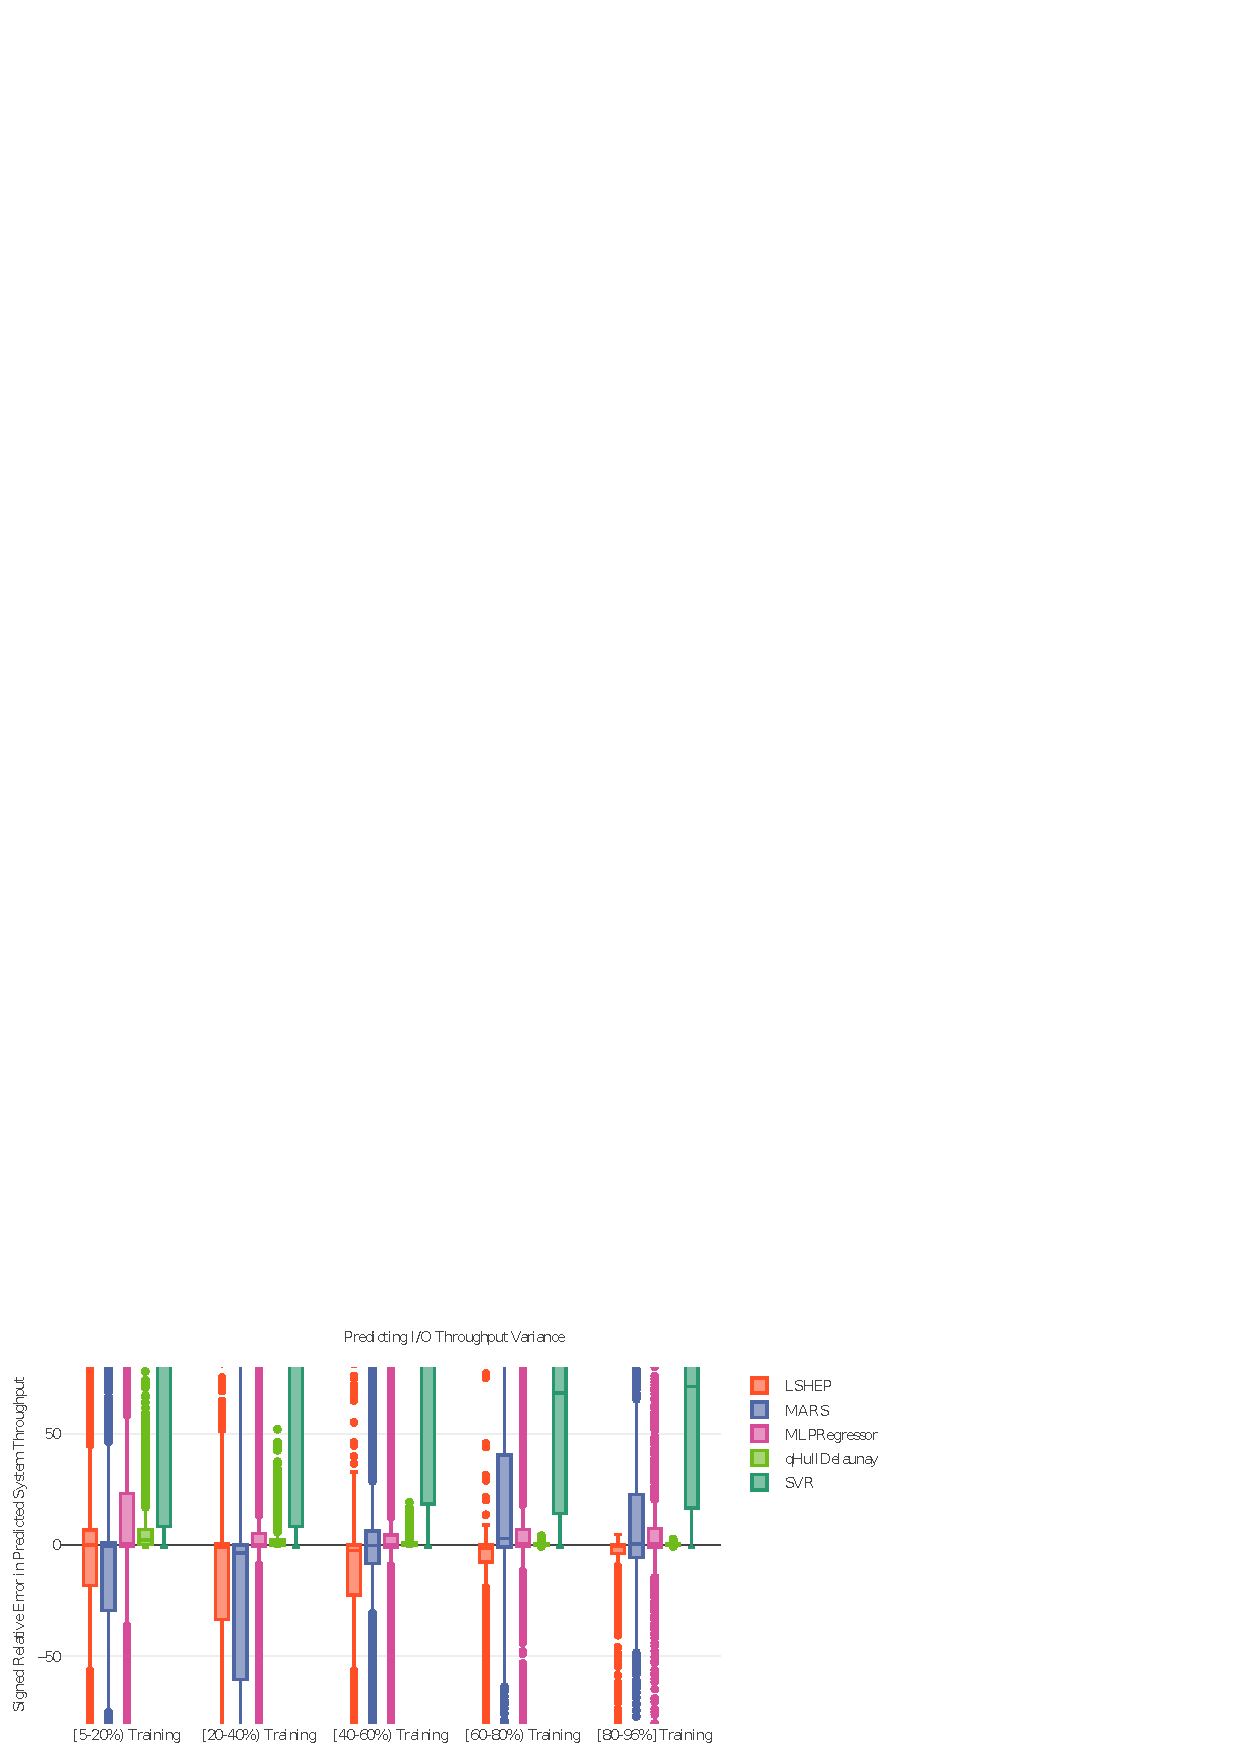
\includegraphics[width=\textwidth,trim={0 .5in 0 .3in}]{Var_TT_Ratio.pdf}
  \caption{These box plots show the prediction error of variance with
    increasing amounts of training data provided to the models. The
    response values being predicted span six orders of magnitude. For
    SVR the top box whisker goes from around 6000 to 400 (decreasing
    by factors of 2) from left to right and is truncated in order to
    maintain focus on better models. Results for all dimensions are
    aggregated. Max training percentage is 96\% due to rounding
    training set size.}
  \label{fig:var_tt_ratio}
\end{figure}
 
\vspace{-10pt}
\subsection{I/O Throughput Variance}
\vspace{-10pt} The prediction results for variance resemble those for
predicting mean. Delaunay remains the best overall predictor
(aggregated across training percentages and dimensions) with median
relative error of .47 and LSHEP closely competes with Delaunay having
a median signed relative error of -.92. Outliers in prediction error
are much larger for all models. Delaunay produces relative errors as
large as 78 and other models achieve relative errors around
$10^3$. The relative errors for many models scaled proportional to the
increased orders of magnitude spanned by the variance response
compared with mean response. As can be seen in Figure
\ref{fig:var_tt_ratio}, all models are more sensitive to the amount of
training data provided than their counterparts for predicting mean.

\vspace{-10pt}
\subsection{Increasing Dimension and Decreasing Training Data}
\vspace{-10pt}
As can be seen in Figure \ref{fig:mean_dim}, all of the models suffer
increasing error rates in higher dimension. This is expected, because
the number of possible interactions to model grows
exponentially. However, LSHEP and Delaunay maintain the slowest
increase in relative error. The increase in error seen for Delaunay
suggests that it is capable of making predictions with a range of
relative errors that grows approximately linearly with increasing
dimension input. This trend suggests that Delaunay would remain a
viable technique for accurately modeling systems with 10's of
parameters given only small amounts of training data. All models, with
the exception of MARS, produce smaller errors given more training
data. Increasing the amount of training data most notably reduces the
number of prediction error outliers.

%     Discussion     
%====================
\section{Discussion}
\label{sec:discussion}

The present results demonstrate that a straightforward application of
multivariate modeling techniques can be used to effectively predict
HPC system performance. Some modeling effort on the part of a systems
engineer combined with a significant amount of experimentation (days
of CPU time for the IOzone data used here) can yield a model capable
of accurately tuning an HPC system to the desired performance
specification, although qualitatively correct predictions can be
achieved with much less (10\%, say) effort.

\vspace{-10pt}
\subsection{Modeling the System}
\vspace{-10pt}
The modeling techniques generated estimates of drastically different
quality when predicting I/O throughput mean and variance. A few
observations: SVR has the largest range of errors for all selections
of dimension and amounts of training data; MARS and LSHEP produce
similar magnitude errors while the former consistently underestimates
and the latter consistently overestimates; Delaunay has considerably
fewer outliers than all other methods. SVR likely produces the poorest
quality predictions because the underlying parametric representation
is global and oversimplified (a single polynomial), making it unable
to capture the complex local behaviors of system I/O. It is still
unclear, however, what causes the behaviors of LSHEP, MARS, and
Delaunay. An exploration of this topic is left to future work.

While the Delaunay method appears to be the best predictor in the
present IOzone case study, it is important to note that the Delaunay
computational complexity increases with the dimension of the input
more rapidly than other techniques. The implementation of Delaunay
(QuickHull) used would experience unacceptably large training times
beyond ten-dimensional input. This leaves much room for other
techniques to perform best in higher dimension unless a more efficient
implementation of Delaunay can be used.

Finally, the ability of the models to predict variance was
significantly worse than for the I/O mean. The larger scale in
variance responses alone do not account for the increase in relative
errors witnessed. This suggests that system variability has a greater
underlying functional complexity than the system mean and that latent
factors are reducing prediction performance.

\vspace{-10pt}
\subsection{Extending the Analysis}
\vspace{-10pt}
System I/O throughput mean and variance are simple and useful system
characteristics to model. The process presented in this work is
equally applicable to predicting other useful performance
characteristics of HPC systems such as: computational throughput,
power consumption, processor idle time, context switches, RAM usage,
or any other ordinal performance metric. For each of these there is
the potential to model system variability as well. This work has
chosen variance as a measure of variability, but the techniques used
in this paper could be applied to more precise measures of variability
such as the percentiles of the performance distribution or the entire
distribution itself. A thorough exploration of HPC systems
applications of multivariate modeling constitutes future work.

%% \begin{enumerate}
%% \item Measuring different system characteristics other than I/O
%% \item Recording system performance constantly to maintain model accuracy
%% \end{enumerate}

\section{Conclusion}
\label{sec:conclusion}
Multivariate models of HPC system performance can effectively predict
I/O throughput mean and variance. These multivariate techniques
significantly expand the scope and portability of statistical models
for predicting computer system performance over previous work. In the
IOzone case study presented, the Delaunay method produces the best
overall results making predictions for 821 system configurations with
less than 5\% error when trained on only 43 configurations. Analysis
also suggests that the error in the Delaunay method will remain
acceptable as the number of system parameters being modeled
increases. These multivariate techniques can and should be applied to
HPC systems with more than four tunable parameters in order to
identify optimal system configurations that may not be discoverable
via previous methods nor by manual performance tuning.

%     Future Work     
%=====================
\vspace{-10pt}
\subsection{Future Work}
\vspace{-10pt}
The most severe limitation to the present work is the restriction to
modeling strictly ordinal (not categorical) system parameters.
Existing statistical approaches for including categorical variables
are inadequate for nonlinear interactions in high dimensions. Future
work could attempt to identify the viability of different techniques
for making predictions including categorical system parameters.

There remain many other multivariate modeling techniques not included
in this work that should be evaluated and applied to HPC performance
prediction. For I/O alone, there are far more than the four tunable
parameters studied in this work. Alongside experimentation with more
models, there is room for a theoretical characterization of the
combined model and data properties that allow for the greatest
predictive power.

%% \color{black}

%% \newpage
%% \ \\

%% \vspace{3in}

%% \texttt{\textbf{L}oc\textbf{A}ll\textbf{Y} li\textbf{NE}ar
%%   \textbf{W}eighted \textbf{A}pproxima\textbf{T}ion\textbf{S}
%%   \textbf{O}f fu\textbf{N}tions}\\
%% %% \texttt{L\ \ A\ \ Y \ \ NE\ \ \  W\ \ \ \ \ \ \ \ A\ \ \ \ \ \ \ \ T\ \ \ S O\ \ \ \ N\ \ \ \ \ \ }
%% \newpage

\bibliographystyle{scsproc}
\bibliography{paper}

\section*{Additional Authors}
Jon Bernard\\
Dept. of Computer Science, VPI \& SU, Blacksburg, VA 24061 \\ [8pt]
Bo Li \\
Dept. of Computer Science, VPI \& SU, Blacksburg, VA 24061\\ [8pt]
Li Xu \\
Dept. of Statistics, VPI \& SU, Blacksburg, VA 24061\\ [8pt]
Godmar Back\\
Dept. of Computer Science, VPI \& SU, Blacksburg, VA 24061\\ [8pt]
Ali R. Butt\\
Dept. of Computer Science, VPI \& SU, Blacksburg, VA 24061\\ [8pt]
Kirk W. Cameron\\
Dept. of Computer Science, VPI \& SU, Blacksburg, VA 24061\\ [8pt]
Yili Hong\\
Dept. of Statistics, VPI \& SU, Blacksburg, VA 24061\\ 

%     Author Biography Block     
%================================
\section*{Author Biographies}

\textbf{\uppercase{Thomas C. H. Lux}} is a Ph.D. student at Virginia Tech
studying computer science under Dr. Layne Watson.

\textbf{\uppercase{Layne T. Watson}} (Ph.D., Michigan, 1974) has interests
in numerical analysis, mathematical programming, bioinformatics, and data
science.
He has been involved with the organization of HPCS since 2000.

\textbf{\uppercase{Tyler H. Chang}} is a Ph.D. student at Virginia Tech
studying computer science under Dr. Layne Watson.

\textbf{\uppercase{Jon Bernard}} is a Ph.D. student at Virginia Tech
studying computer science under Dr. Kirk Cameron.

\textbf{\uppercase{Bo Li}} is a senior Ph.D. student at Virginia Tech
studying computer science under Dr. Kirk Cameron.

\textbf{\uppercase{Li Xu}} is a Ph.D. student at Virginia Tech studying
statistics under Dr. Yili Hong.

\textbf{\uppercase{Godmar Back}} (Ph.D., University of Utah, 2002) has
broad interests in computer systems, with a focus on performance and
reliability aspects of operating systems and virtual machines.

\textbf{\uppercase{Ali R. Butt}} (Ph.D., Purdue, 2006) has interests in cloud computing, distributed computing, and operating system induced variability.

\textbf{\uppercase{Kirk W. Cameron}} (Ph.D., Louisiana State, 2000) has
interests in computer systems design, performance analysis, and power and
energy efficiency.

\textbf{\uppercase{Yili Hong}} (Ph.D., Iowa State, 2009) has interests in
engineering statistics, statistical modeling, and data analysis.

\end{document}
